\section{Introduction}
This paper uses CYCLUS, the agent-based simulator \cite{huff_fundamental_2016} to analyze
the future nuclear inventory in the European Union. This paper focuses on the spent fuel
inventory in the EU nations in 2050, and analyzes various potential strategies of spent fuel
management.
A major focus of this paper is to determine the extent to which France has an incentive
to receive all the \gls{SNF} from EU nations to create \gls{MOX}.
The \gls{MOX} created will fuel French transition to a \gls{SFR} fleet
and may allow France to avoid building additional \glspl{LWR}.
A CYCLUS simulation is run to calculate
how much spent fuel is created from EU nations from 1970 to 2050, as well as the amount
of \gls{MOX} that can be created with the \gls{SNF} inventory.
The paper assumes a once-through cycle for all 
EU nations with the exception of France. France can reprocess spent \gls{UOX} and \gls{MOX} to
produce \gls{MOX} from reprocessed plutonium and depleted uranium (tails).
The simulation assumes \gls{MOX} is reprocessed infinitely. 
After obtaining the \gls{SNF} inventory of all EU in 2050, a separate
simulation is run where the \gls{SNF} inventory is reprocessed and
used as fuel for the newly deployed \gls{SFR} reactors.
\gls{SFR} reactors are reactors that use \gls{MOX} fuel to a burnup
of approximately 100 GWdth/t. This allows enough production of plutonium
for an equivalent mass of \gls{MOX}, if mixed with tailings.  Eventually,
the used \gls{UOX} inventory will be exhausted, and the \glspl{SFR} must be
fueled by \gls{MOX} created from recycled \gls{MOX}.
It is assumed that \glspl{SFR} are available for deployment
from 2040. 


\section{Methodology}
The work relies on CYCLUS, an agent-based simulator, to simulate the nuclear fuel cycle
and track material flows in EU nations. An open-source database from \gls{IAEA} called
\gls{PRIS} is imported as a csv file, listing the country, reactor unit, type, net capacity (MWe), status,
operator, construction date, first criticality date, first grid date, commercial date, shutdown
date (if applicable), and unit capacity factor for 2013. Then only the EU countries are extracted
from the csv file. A python script is written up to generate a CYCLUS input file from the csv file,
which lists the individual reactor units as agents. After running the CYCLUS input file,
the output file is analyzed by another python script.

First, a simulation is run from 1970 to 2050 to calculate the mass of 
\gls{SNF} and depleted uranium (tails) EU accumulates before 2050. 
The second simulation uses the \gls{SNF} inventory from the previous
simulation to calculate the mass of the \gls{SNF} inventory can fuel
the newly deployed \gls{SFR}s. French \gls{SFR}s are deployed
to make up for the decommissioned capacity of \gls{LWR}s.


\section{Time Scope and Future Projections}
Projections of future reactor deployment in this simulation were
assessed based on analysis from references \gls{PRIS},
\cite{world_nuclear_2017} \cite{joskow_future_2012} \cite{hatch_politics_2013}.
The projections extend to 2050 at the latest. This allows the simulation to take place from
1970 to 2050, the latest foreseeable future. The specific plans for each EU nation are explained
in detail in later sections.

It is also assumed that all reactors that are 
currently operating have a lifetime of 60 years, unless their government plans
early shutdown. This will approximate when and how much \glspl{SFR} need to be built
to make up for the shutdown of \glspl{LWR}.


\subsection{Depletion Calculations}
Depletion calculations of the nuclear fuel are done
naively, with a model burnup depletion recipe (mass fraction) used
for each reactor type, and the mass of the fuel 
adjusted linearly with capacity. For example, a PWR of
1,000 MWe capacity has 193 assemblies of 3.2\% enriched
uranium fuel, with each assembly with a mass of 523.4 kg.
The core has a 18 month cycle, where one-third of the 
core (64 assemblies) are discharged per refueling. The refueling
is assumed to take 2 months to complete, during which the reactor
is shut down. For the \gls{SFR}, a model design is adopted from
MARSAULT–Marie-Sophie et al. \cite{marsault-marie-sophie_pre-conceptual_2012}.

For the compositions of the fuel, a reference depletion calculation
from ORIGEN is used (see appendix). The recipe has also been used for
\cite{wilson_adoption_2009}.

\subsection{French \gls{SFR} Deployment Schedule}

From 2040, when \gls{SFR}s become available,
600-MWe \gls{SFR}s are deployed to make up for the 
decommissioned \gls{LWR} capacities.

Initially, in 2040, 22 \gls{SFR}s
are deployed for the previously decommissioned
\gls{LWR}s. This results in an installed capacity of 60,000 MWe
of \gls{SFR} by 2076.

\begin{table}[h]
	\centering
	\label{tab:sfr_deploy}
	\caption{French SFR Deployment Schedule to Maintain Installed Capacity}
	\begin{tabular}{|c|c|c|c|}	
		\hline
		Months from 1970 & Decommissioned Capacity [MWe] & \gls{SFR}s Deployed & \gls{SFR} Capacity [GWe] \\ \hline
		Total & 51,700 & 86 &  60\\ \hline
		841 & NA & 22 & 13.2 \\ \hline
		842 & 915 & 2 & 14.4 \\ \hline
		847 & 915 & 1 & 15 \\ \hline
		851 & 915 & 2 & 16.2 \\ \hline
		852 & 915 & 2 & 17.4 \\ \hline
		853 & 890 & 1 & 18 \\ \hline
		856 & 915 & 2 & 19.2 \\ \hline
		857 & 915 & 1 & 19.8 \\ \hline
		859 & 890 & 2 & 21 \\ \hline
		870 & 910 & 1 & 21.6 \\ \hline
		874 & 905 & 2 & 22.8 \\ \hline
		879 & 915 & 1 & 23.4 \\ \hline
		880 & 910 & 2 & 24.6 \\ \hline
		883 & 910 & 1 & 25.2 \\ \hline
		885 & 905 & 2 & 26.4 \\ \hline
		891 & 1330 & 2 & 27.6  \\ \hline
		894 & 1330 & 2 & 28.8 \\ \hline
		895 & 915 & 2 & 30. \\ \hline
		897 & 915 & 1 & 30.6 \\ \hline
		906 & 1335 & 2 & 31.8 \\ \hline
		907 & 910 & 2 & 33. \\ \hline
		908 & 1330 & 2 & 34.2 \\ \hline
		914 & 1330 & 2 & 35.4 \\ \hline
		916 & 1335 & 2 & 36.6 \\ \hline
		921 & 1300 & 3 & 38.4 \\ \hline
		930 & 1300 & 2 & 39.6 \\ \hline
		931 & 1310 & 2 & 40.8 \\ \hline
		933 & 905 & 2 & 42. \\ \hline
		940 & 1310 & 2 & 43.2 \\ \hline
		944 & 1310 & 2 & 44.4 \\ \hline
		960 & 1300 & 2 & 45.6 \\ \hline
		962 & 1330 & 2 & 46.8 \\ \hline
		963 & 1310 & 2 & 48. \\ \hline
		975 & 1300 & 3 & 49.8 \\ \hline
		983 & 1330 & 2 & 51. \\ \hline
		1000 & 1310 & 2 & 52.2 \\ \hline
		1038 & 1500 & 2 & 53.4 \\ \hline
		1045 & 1500 & 3 & 55.2 \\ \hline
		1054 & 1495 & 3 & 57. \\ \hline
		1078 & 1495 & 2 & 58.2 \\ \hline
		1283 & 1600 & 3 & 60. \\ \hline
		
		\end{tabular}
\end{table}


\begin{figure}[htbp!]
	\begin{center}
		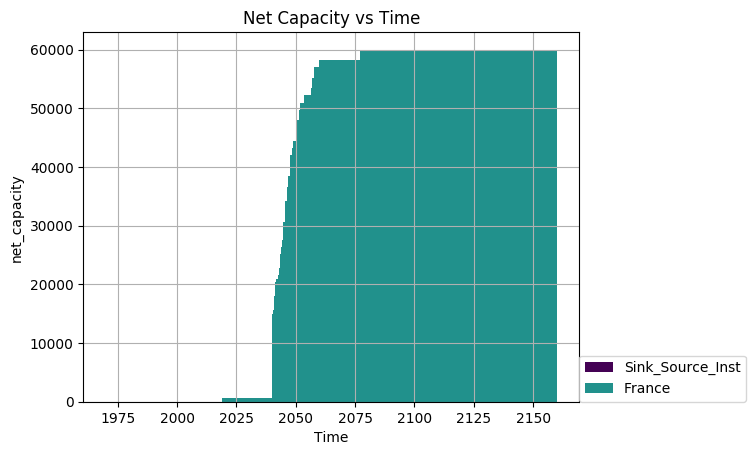
\includegraphics{./images/power_plot.png}
	\end{center}
	\caption{Timeseries of installed capacity of \gls{SFR}s}
	\label{fig:sfr_cap}
\end{figure}


\begin{figure}[htbp!]
	\begin{center}
		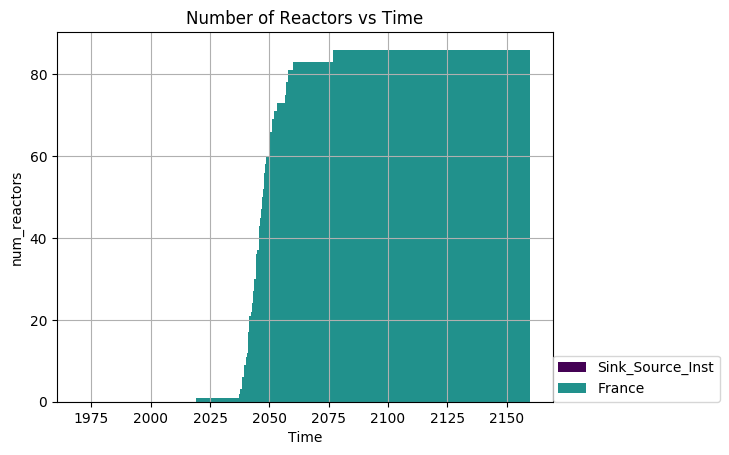
\includegraphics{./images/number_plot.png}
	\end{center}
	\caption{Timeseries of number of \gls{SFR}s}
	\label{fig:sfr_num}
\end{figure}



\subsection{Scenario Descriptions}
The simulation follows the model fuel cycle, where a `source'
provides natural uranium, which is enriched by an 'enrichment'
facility to \gls{UOX}, while disposing enrichment waste (tailings)
to the 'sink' facility. The enriched \gls{UOX} is used
in the \gls{LWR}s and \gls{UOX} waste is produced. The spent fuel
is then reprocessed to separate plutonium and uranium.
The plutonium is mixed with depleted uranium (tails) to \gls{MOX}.
The reprocessed uranium is stockpiled. \gls{SNF} decay is assumed
to have no effect on reprocessing viability.

The second scenario estimates the \gls{SNF} inventory in EU at 2050,
and reprocesses the \gls{SNF} to separate plutonium. The separated
plutonium is mixed with the depleted uranium inventory from 2050
to create \gls{MOX}, which is used in the \gls{SFR}s. The used
\gls{MOX} is also reprocessed to extract plutonium, which also
is mixed with depleted uranium to produce \gls{MOX}.



\subsection{Reprocessed Uranium}
Reprocessed uranium contains a range of uranium isotopes, from $^{232}U$ to $^{238}U$.
This brings complications in reusing reprocessed uranium as a fuel source \cite{IAEA_management_2007}.
The presence of neutron-absorbing isotopes $^{234}U$ and $^{236}U$ requires reprocessed uranium
to require a higher enrichment of $^{235}U$. There is trace amounts (2 ppb) of fissile istope $^{233}U$,
which provides little benefit.  
Also, $^{232}U$ has a decay chain of short-lived
daughter products that undergo intense beta and gamma radiation.
The French nuclear program utilizes a fraction (1/3) of reprocessed uranium as fuel \cite{IAEA_management_200&}.
However for this simulation the reprocessed uranium is simply stockpiled.


